---
id: tkz-euclide-ejemplo-54
title: "Ángulo obtuso"
description: "Creación de un ángulo obtuso"
keywords: [angulo,obtuso,rayo,taller1]
tags: [tkzDefShiftPoint,tkzFillAngle,tkzMarkAngle,tkzDrawLines]
sort: 54
---
\documentclass[tikz,border=2mm]{standalone}
\usepackage{xcolor}
\usepackage{tkz-base}
\usepackage{tkz-euclide}

\begin{document}
    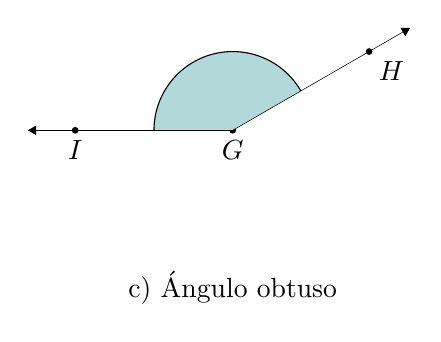
\begin{tikzpicture}                
        % Paso 1: Define vértice del ángulo
        \tkzDefPoint(13,2){G}

        % Paso 2: Define punto del rayo inferior a 30° de G
        \tkzDefShiftPoint[G](30:2){H}
        
        % Paso 3: Define punto del rayo inferior a 180° de G
        \tkzDefShiftPoint[G](180:2){I}

        % Paso 4: Dibuja los puntos y etiquétalos
        \tkzDrawPoints(G,H,I)        
        \tkzLabelPoints[below right](H)
        \tkzLabelPoints[below](I,G)

        % Paso 5: Marca y rellena el ángulo
        \tkzFillAngle[fill=teal!30](H,G,I)
        \tkzMarkAngle(H,G,I)

        % Paso 6: Dibuja los segmentos de los rayos
        \tkzDrawLines[add=0 and 0.3, -Triangle](G,H G,I)

        % Paso 7: Describe cada ejemplo        
        \tkzText(13,0){c) Ángulo obtuso}
    \end{tikzpicture}
\end{document}
